\documentclass[border=10pt]{standalone}

\usepackage{tikz}
\usepackage{tikzsymbols}
\usetikzlibrary{calc,patterns,shapes.geometric}

\def\centerarc[#1](#2)(#3:#4:#5){\draw[#1] ($(#2)+({#5*cos(#3)},{#5*sin(#3)})$) arc (#3:#4:#5);}

\begin{document}
	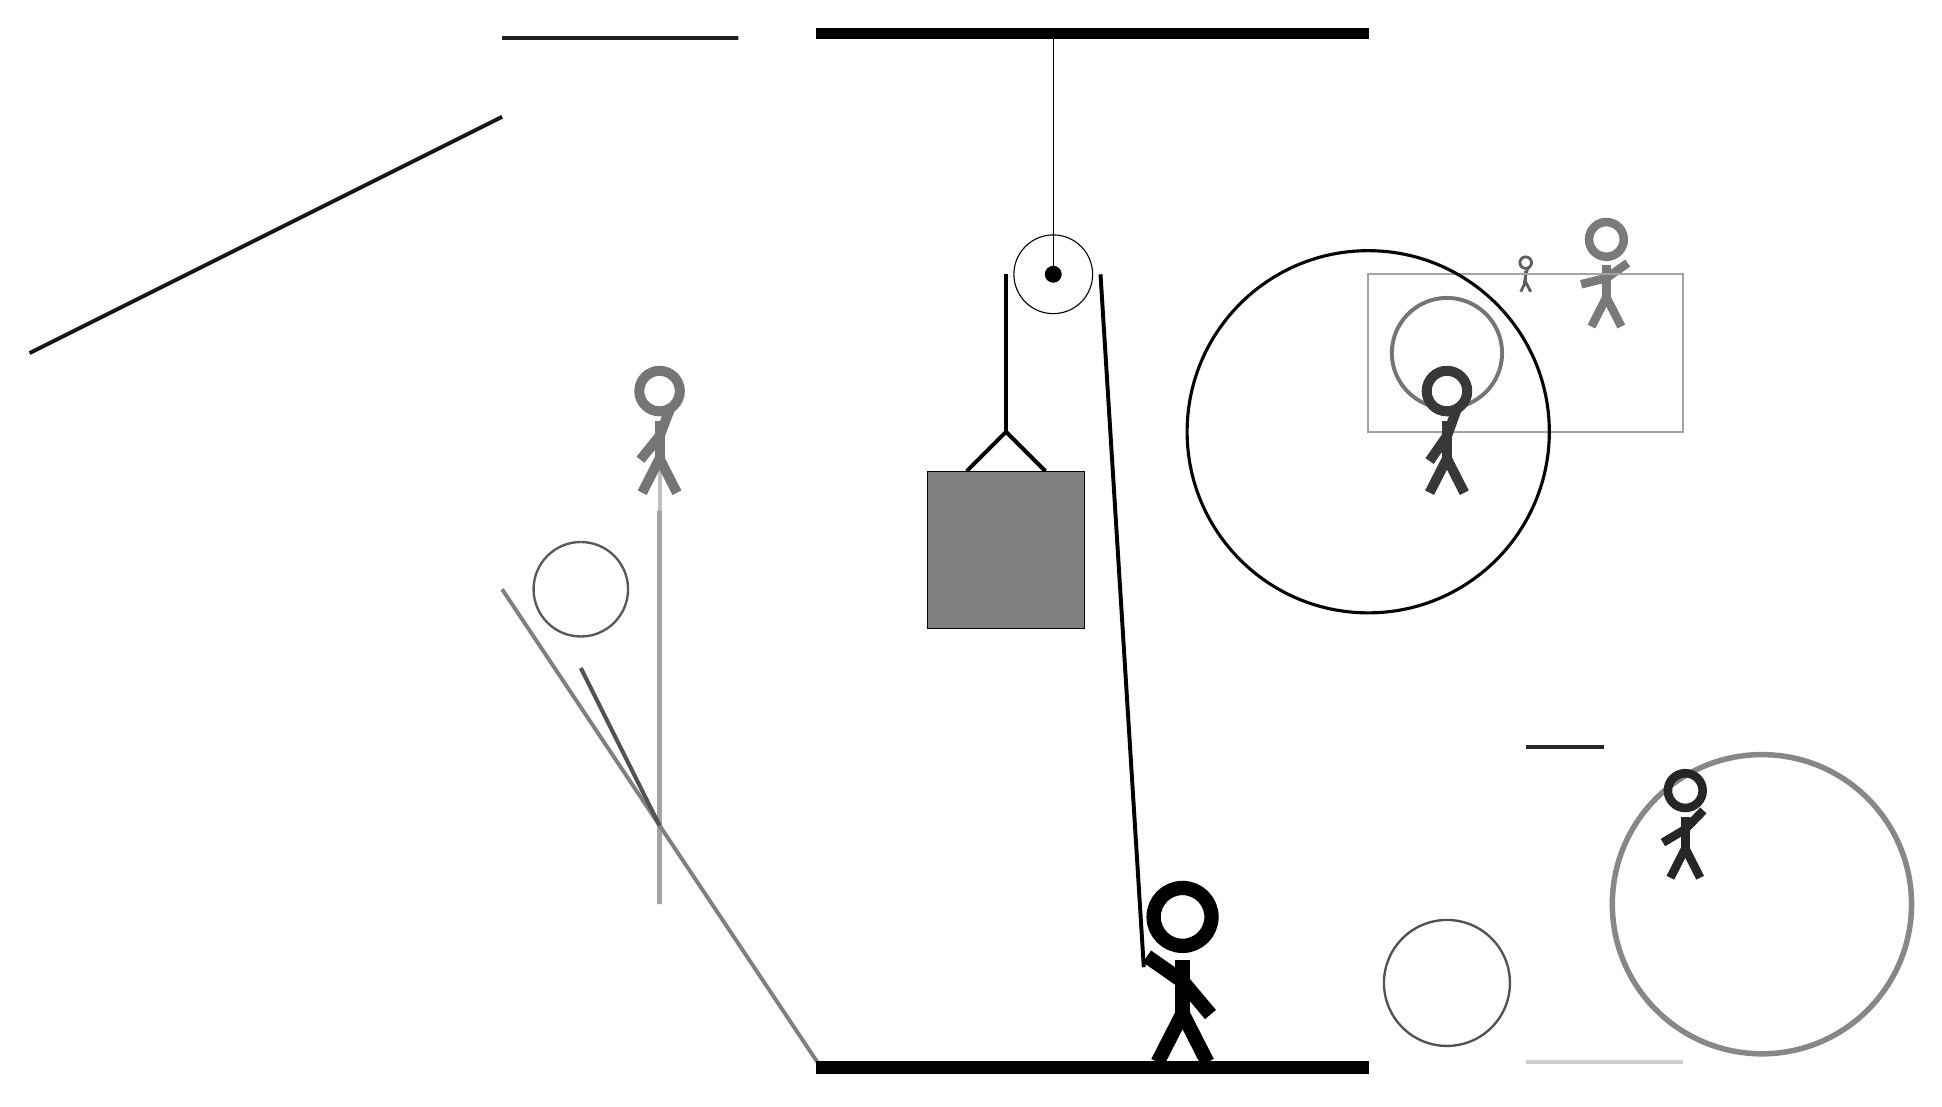
\begin{tikzpicture}
		%%%%% START %%%%%
		
		\draw[fill=black] (-2, 10) rectangle (5, 10.125);
		
		\draw (1, 7) circle (0.5);
		\draw[fill=black] (1, 7) circle (0.1);
		\draw (1, 10) -- (1, 7);
		
		\draw[line width=0.5mm] (-0.1, 4.5) -- (0.4, 5.0) -- (0.9, 4.5);
		\draw[fill=black!50] (-0.6, 4.5) rectangle (1.4, 2.5);
		
		\draw[line width=0.5mm] (0.4, 7) -- (0.4, 5.0);
		\centerarc[line width=0.5mm](1, 7)(0:180:0.6);
		\draw[line width=0.5mm](1.6, 7) -- (2.15, -1.8);
		
		\node at (2.6, -1.9) {\Strichmaxerl[10][-35][-50]};
		
		\draw[line width=0.5mm, color=black!25](-4, 2) -- (-4, 5);
		
		\draw[line width=0.6mm, color=black!36] (-4, 4) rectangle (-4, -1);
		\draw[line width=0.5mm, color=black!19](9, -3) -- (7, -3);
		\draw[line width=0.5mm, color=black!84](8, 1) -- (7, 1);
		
		\draw [line width=0.7mm, color=black!47](10, -1) circle (1.9);
		
		\node[line width=0.4mm, color=black!63] at (7, 7) {\Strichmaxerl[2][80][75]};
		
		\draw [line width=0.5mm, color=black!54](6, 6) circle (0.7);
		\draw[line width=0.4mm, color=black!87] (-3, 10) rectangle (-6, 10);
		\draw[line width=0.5mm, color=black!50](-2, -3) -- (-6, 3);
		\draw[line width=0.5mm, color=black!91](-6, 9) -- (-12, 6);
		
		\draw[line width=0.5mm, color=black!68](-5, 2) -- (-4, 0);
		\node[line width=0.7mm, color=black!54] at (-4, 5) {\Strichmaxerl[7][51][69]};
		\draw [line width=0.3mm, color=black!68](6, -2) circle (0.8);
		
		\node[line width=0.3mm, color=black!52] at (8, 7) {\Strichmaxerl[6][14][35]};
		\draw[line width=0.3mm, color=black!36] (5, 5) rectangle (9, 7);
		\node[line width=0.4mm, color=black!85] at (9, 0) {\Strichmaxerl[6][31][46]};
		\draw [line width=0.3mm, color=black!65](-5, 3) circle (0.6);
		
		\node[line width=0.6mm, color=black!78] at (6, 5) {\Strichmaxerl[7][55][70]};
		\draw [line width=0.4mm, color=black!98](5, 5) circle (2.3);
		
		\draw[fill=black] (-2, -3) rectangle (5, -3.15);
		
		%%%%% END %%%%%
	\end{tikzpicture}
\end{document}